\chapter{Les normes et le raisonnement juridique}
\section{Hiérarchie des normes}
\subsection{Définition}
\large{
\textbf{Le droit} est un ensemble de \textbf{règles} qui organisent la vie en société et régissent \textbf{les relations entre les individus, les institutions et l'état.}
Ces règles sont créées par des \textbf{autorités compétentes}, comme le législateur, et sont appliquées par des tribunaux ou d'autres institutions de justice \newline

Le droit est divisé en plusieurs branches, comme : \newline

}
\begin{itemize}
    \item \textbf{Le droit civil} : concerne les relations entre les particuliers, par exemple en matière de mariage, de propriétés ou de contrats
    \item \textbf{Le droit pénal} : détermine les infractions (crimes, délits, contraventions) et fixe les sanctions applicables
    \item \textbf{Le droit administratif} : encadre les relations entre les citoyens et les administrations publiques
    \item \textbf{Le droit internationnal} : régit les relations entre les états et questions juridiques dépassant les frontières nationnales
    \item \textbf{Le droit commercial} : concerne les activités économiques, les entreprises et les transactions commerciales
\end{itemize}
En cas de non respect de ces règles, le citoyen encours des sanctions. Le droit peut évoluer dans le temps en fonction des changements sociaux, technologiques ou économiques
\begin{center}
    \begin{figure}[hbt!]
        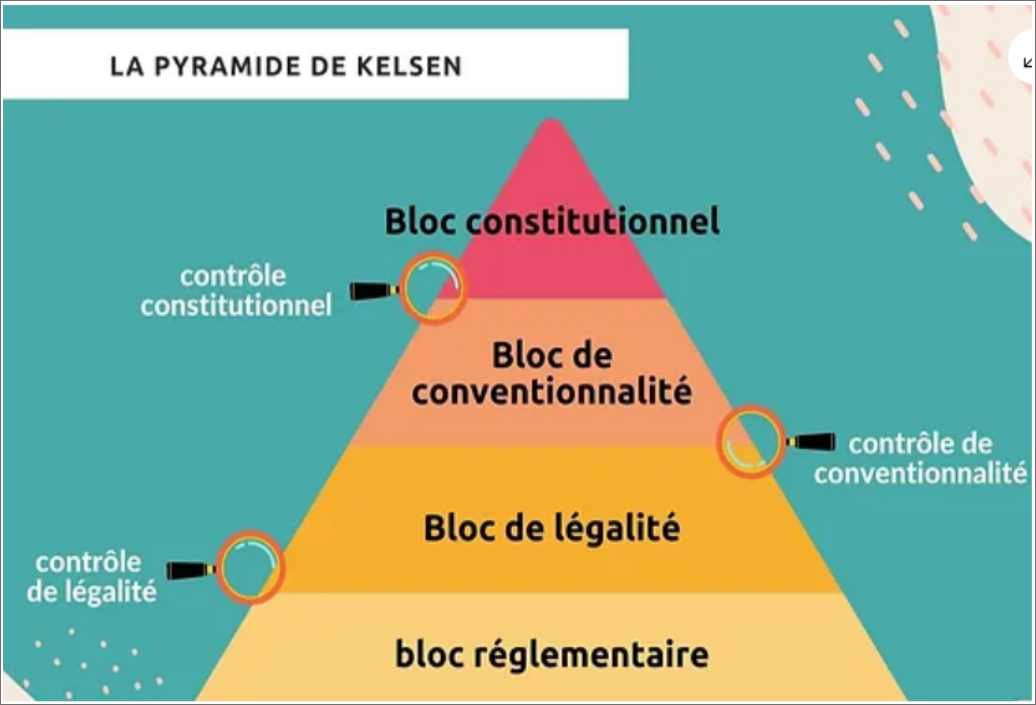
\includegraphics[scale=0.4]{Pics/Pyramide_de_Kelsen.png}
        \caption{Hiérarchie des normes}
    \end{figure}
\end{center}
\newpage
\section{Les normes}
Les \textbf{normes juridiques} sont à différentier des \textbf{normes sociales}. Une norme juridique est une règle qui établit une source de droits et d'obligations juridiques tandis
qu'une norme sociale provient d'une tradition, de la morale lorsqu'un individu se socialise. 
\subsection{Bloc constitutionnel}
C'est la Constitution : un ensemble de normes juridiques, de principes et de règles appliquées par le conseil constitutionnel. \footnote{Vérifie la conformité des lois à la Constitution}
\begin{center}
    \begin{figure}[hbt!]
        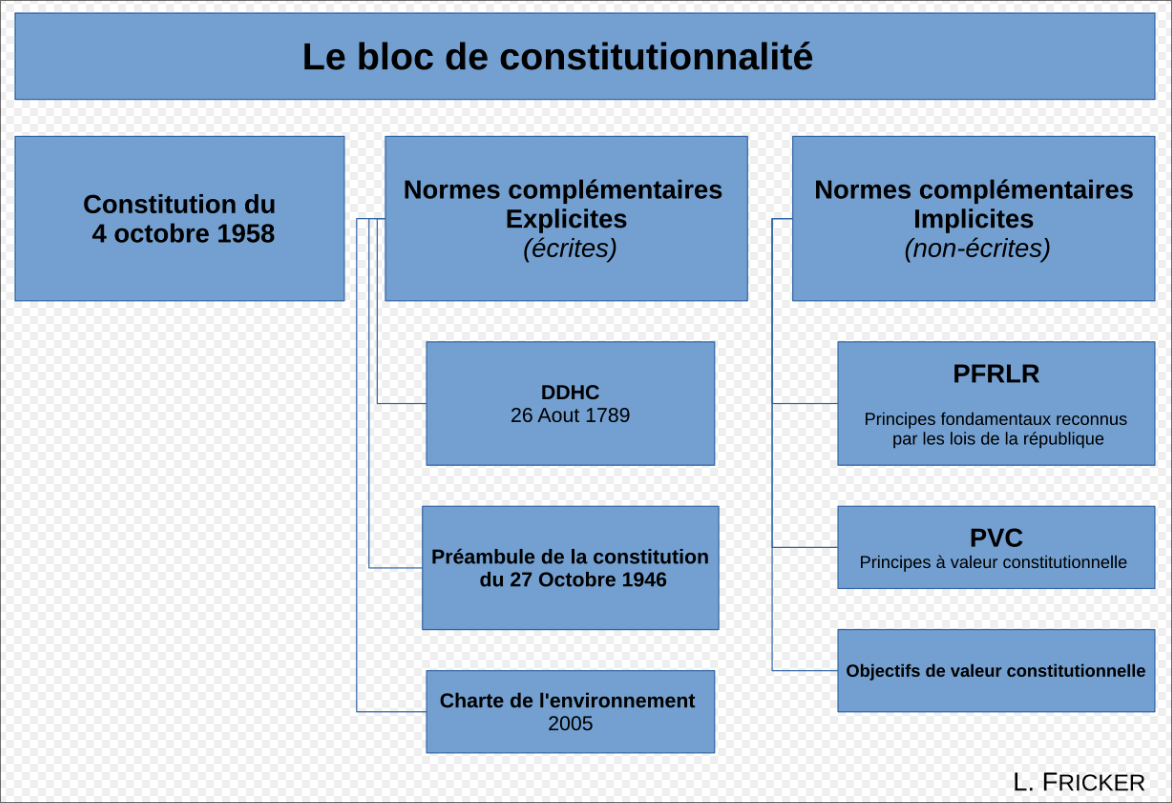
\includegraphics[scale=0.3]{Pics/Bloc_de_constitutionnalite.png}
        \caption{Bloc constitutionnel}
    \end{figure}
\end{center}
\newpage
\subsection{Bloc conventionnel}
\textbf{Le bloc de conventionnalité l'ensemble des traités et conventions entre les Etats ou entre mes Etats et les organisations internationnales} \newline
Exemple : l'\textbf{UE} est une organisation économique et politique qui rasssemble 27 états membres. Elle a pour but de promouvoir la paix, la stabilité et la coopération économique entre les états memebres. \newline
\begin{center}
    \begin{figure}[hbt!]
        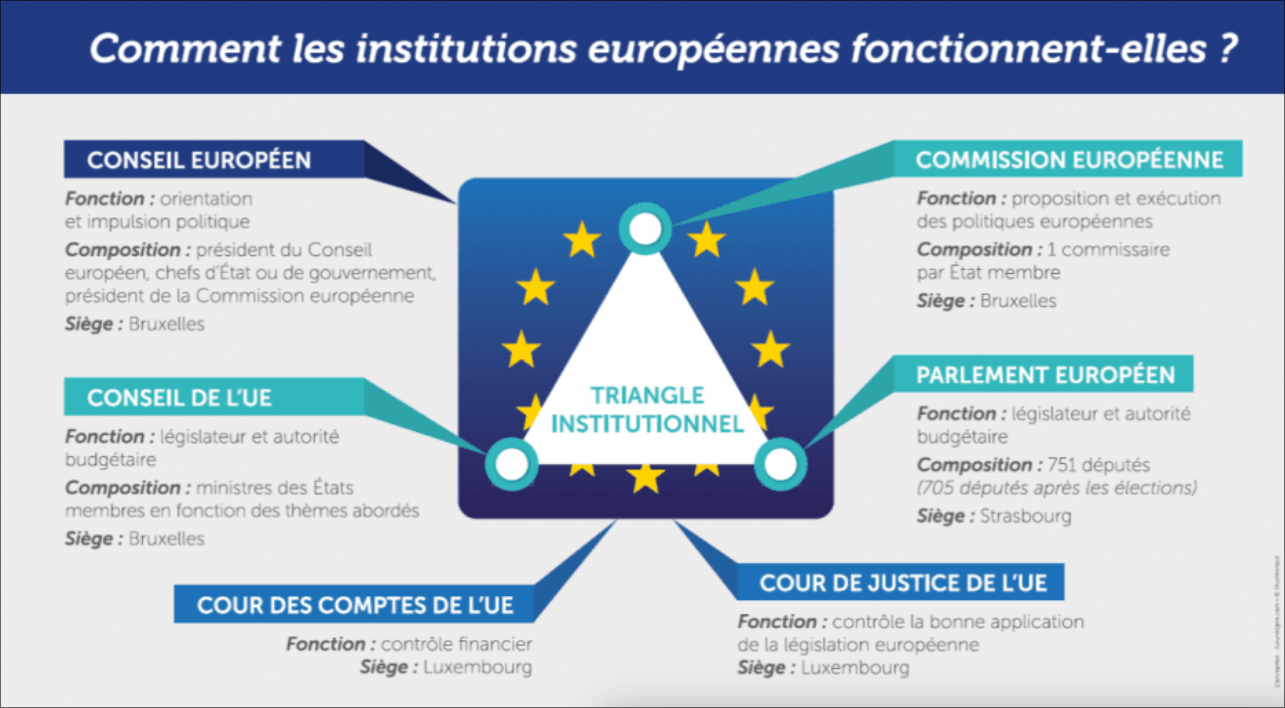
\includegraphics[scale=0.3]{Pics/Institutions_UE.png}
        \caption{Illustration des institutions dans l'Union Européenne}
    \end{figure}
\end{center}
\newpage
\subsection{Bloc}
\newpage
\chapter{Annexe sur les institutions de l'UE et ses principes}
\newpage
\section{L'UE et ses institutions}
Exemple de traités fondateurs :
\begin{itemize}
    \item Communauté Européenne de charbon et de l'acier (CECA) 1951 qui réunit les pays fondateurs de l'UE : l'Allemagne, l'Italie, la France, le Luxembourg, les Pays Bas et la Belgique
    \item Communauté Economique Européenne (CEE), traité de Rome 
    \item Communauté Européenne de l'Energie Atomique (EURATOM), 1957 \newline
\end{itemize}

Institutions principales : 
\begin{itemize}
    \item La commission européenne : propose les lois et veille à leurs applications
    \item Le parlement européen : représente la voix des citoyens
    \item Le conseil de l'UE : représente les Etats et co-légifère avec le parlement
    \item Le conseil Européen : réunion des chefs d'Etat pour donner les orientations politiques
    \item La cour de justice de l'UE : veille à l'interprétation et l'application du droit européen \newline
\end{itemize}

\newpage
Politiques clés :
\begin{itemize}
    \item Le climat
    \item La sécurité
    \item Les droits sociaux et l'égalité \newline
\end{itemize}

Traités :
\begin{itemize}
    \item Traité sur l'UE
    \item EURATOM
    \item \textbf{Traité sur le Fonctionnement de l'Union Européenne (TFUE)} \newline
\end{itemize}
\newpage
\section{Principe de subsidiarité}
Permet de déterminer le niveau d'intervention le plus pertinant des états membres pour la mise en place des actions envisagées
\newline
\section{Compétences partagées}
Les états membres de l'UE peuvent partager leurs Compétences afin de réaliser une action (ex : aider un pays en crise) \newline
Les compétences partagées concernent :
\begin{itemize}
    \item Le marché intérieur
    \item La politique sociale
    \item La cohésion économique, sociale et territoriale
    \item L'agriculture et la pêche
    \item L'environement
    \item La protection des consommateurs
    \item Le transport
    \item Les réseaux transeuropéens
    \item L'énergie
    \item L"espace de liberté, de sécurité et de justice
    \item La santé publique
    \item La recherche, le développement et l'espace
    \item L'aide humanitaire \newline
\end{itemize}
\newpage
\section{Principe de solidarité}
Les états membres doivent assurer la mise en balance des intérêts de l'UE en fonction de leurs compétences en prennant en compte la viabilité économique et politique de leurs agissement, autant pour eux-mêmes que pour les autres états membres
\section{Exemple : La concurrence du secteur de l'électricité en Europe}
\subsection{Ouverture à la concurrence}
\subsubsection{1er paquet}
\begin{itemize}
    \item Directive 96/92 du 19 décembre 1996 concernant des règles communes pour le marché intérieur de l’électricité
\end{itemize}
\subsubsection{2ème paquet}
\begin{itemize}
    \item Directive 2003/54 du 26 juin 2003 concernant des règles communes pour le marché intérieur de l’électricité
    \item Règlement 1228/2003 du 26 juin 2003 sur les conditions d’accès au réseau pour les échanges transfrontaliers d’électricité
\end{itemize}
\subsubsection{3ème paquet}
\begin{itemize}
    \item Directive 2009/72 du 13 juillet 2009 concernant des règles communes pour le marché intérieur de l’électricité
    \item Règlement 713/2009 du 13 juillet 2009 instituant une agence de coopération des régulateurs de l’énergie
    \item Règlement 714/2009 du 13 juillet 2009 sur les conditions d’accès au réseau pour les échanges transfrontaliers d’électricité
\end{itemize}
\newpage
\subsection{Le développement des EnR}
\begin{itemize}
    \item Directive 2001/77 du 27 septembre 2001 relative à la promotion de l’électricité produite à partir de sources d’énergie renouvelables sur le marché intérieur de l’électricité
    \item Directive 2009/28 du 23 avril 2009 relative à la promotion de l’utilisation de l’énergie produite à partir de sources renouvelables 
\end{itemize}
\subsection{L'éfficacité énergétique}
\begin{itemize}
    \item Directive 2002/91 du 16 décembre 2002 sur la performance énergétique des bâtiments
    \item Directive 2010/31 du 19 mai 2010 sur la performance énergétique des bâtiments
    \item Directive 2012/27 du 25 octobre 2012 relative à l’efficacité énergétique
\end{itemize}
\subsection{Lutte contre les GES}
\begin{itemize}
    \item Directive 2003/87 du 13 octobre 2003 établissant un système d’échange de quotas d’émission de gaz à effet de serre dans la Communauté
\end{itemize}
\section{Un découpage en 4 parties}
\begin{itemize}
    \item La production - Concurrence
    \item Le transport (RTE) - Activités régulées \textcolor{BrickRed}{Défaillance de marché : monopole naturel}
    \item La distribution (Enedis) - Activités régulées \textcolor{BrickRed}{Défaillance de marché : monopole naturel}
    \item La fourniture de l'électricité - Concurrence
\end{itemize}
\newpage
\section{Différence entre loi et réglement}
\subsection{Nature}
\begin{itemize}
    \item \textbf{Loi} : C'est une norme juridique adoptée par le Parlement. Elle a une portée générale et s'applique à l'ensemble de la population. Les lois sont souvent le résultat de débats parlementaires et peuvent traiter de sujets variés, allant des droits fondamentaux aux questions économiques.
    \item \textbf{Règlement} : C'est une norme juridique édictée par une autorité administrative (gouvernement, ministère, collectivité locale, etc.) pour préciser ou appliquer une loi. Les règlements ont généralement un champ d'application plus restreint et peuvent traiter de détails techniques ou pratiques.
\end{itemize}
\subsection{Processus d'élaboration}
\begin{itemize}
    \item \textbf{Loi} : Pour qu'une loi soit adoptée, elle doit passer par plusieurs étapes, notamment la rédaction, la discussion, l'amendement et le vote au sein des deux chambres du Parlement (dans le cas de la France, l'Assemblée nationale et le Sénat).
    \item \textbf{Règlement} : Les règlements peuvent être adoptés plus rapidement et sans passer par un processus parlementaire aussi complexe. Ils sont souvent le résultat d'une simple décision administrative, bien que certaines procédures de consultation puissent être requises.
\end{itemize}
\subsection{Portée}
\begin{itemize}
    \item \textbf{Loi} : Les lois ont une valeur supérieure et priment sur les règlements en cas de conflit. Elles établissent des principes et des droits fondamentaux.
    \item \textbf{Règlement} : Les règlements doivent respecter les lois dont ils dérivent. Ils précisent les modalités d'application de ces lois et peuvent être modifiés plus facilement.
\end{itemize}